\documentclass[12pt,a4paper]{report}
\usepackage[utf8]{inputenc}
\usepackage[T1]{fontenc}
\usepackage{amsmath}
\usepackage{amsfonts}
\usepackage[english,russian]{babel}
\usepackage{amssymb}
\usepackage{graphicx}
\graphicspath{{pictures/}}
\DeclareGraphicsExtensions{.pdf,.png,.jpg}

\usepackage{hyperref}

\begin{document}
	\begin{center}
		{\large\bf УЧЕБНАЯ ПРАКТИКА.\\
			ПРАКТИКА ПО ПОЛУЧЕНИЮ ПЕРВИЧНЫХ  ПРОФЕССИОНАЛЬНЫХ УМЕНИЙ И НАВЫКОВ, В ТОМ ЧИСЛЕ ПЕРВИЧНЫХ УМЕНИЙ И НАВЫКОВ НАУЧНО-ИССЛЕДОВАТЕЛЬСКОЙ ДЕЯТЕЛЬНОСТИ}\\
		{\it Новиков Е.А.}
	\end{center}
	
	\newpage
	
	\section{Работа, проделанная в период 30.10.2020 - 5.11.2020}
	3.11.2020 Осуществил разбор первой главы книги Наоми Седер "Python. Экспресс-курс". Шло повествовании о плюсах и минус языка Python. Рассказывалось, для чего он полезен и как вынести из него максимальную выгоду. Перешёл ко второй главе. В ней стали описывать "лёгкую" разработку программ в python. Установил PyCharm. Добавил переменные среды. Столкнулся с проблемой некомпилируемой обработки программы ">>> print("Hello, World")". Ошибка 9009. Попытался разобраться сам. Проблема не решилась после переустановки и новой переменной среды. Начал поиск в интернете. Нечего нового не нашёл.

	4.11.2020 Вновь попытался найти полезную информацию в Интернете. Ещё раз переустановил PyCharm. ToolBox перестал его запускать, а только предлагает его переустановить. PyCharm запускается единственным способом - через панель меню "Пуск". Закончил разбор второй главы книги Наоми Седер "Python. Экспресс-курс".
	
	\section{Работа, проделанная в период 06.11.2020 - 12.11.2020}
	9.11.2020 Освоил главу 3. Понял, что знак ">>>" относится к консоли python, а не к коду. Начал главу 4.

	10.11.2020 Дочитал главу 4, сделал задания для лучшего освоения. \url{https://yadi.sk/d/7tAiVBXUr4HP0g?w=1}. Просмотрел лекции Введение, "Искусственные нейронные сети", "Обучение нейронных сетей".

	11.11.2020 Освоил главу 5. Не смог найти файл с лабораторной работы в конце этой главы. \url{https://yadi.sk/d/YZpACJ_52mXBFA?w=1(5.3?)}. Лекции "Библиотеки для глубокого обучения", "Распознавание предметов одежды", "Анализ качества обучения нейронной сети".
	
	\section{Работа, проделанная в период 13.11.2020 - 20.11.2020}
	Определение 

Нейросеть  - это модель обработки информации, которая призвана автоматизировать, упрощать и ускорять работу человека. Она действует так же, как и биологические нервные системы человека, созданные для обработки информации. 

 Типы нс: 

\begin{enumerate}
\item Сверточные сети - одни из самых популярных типов искусственных нейронных сетей. Они доказали свою эффективность в распознавании визуальных образов (видео и изображения), рекомендательных системах и обработке языка.

Сверточные нейронные сети отлично масштабируются и могут использоваться для распознавания образов, какого угодно большого разрешения.
В этих сетях используются объемные трехмерные нейроны. Внутри одного слоя нейроны связаны лишь небольшим полем, названые рецептивным слоем.
Нейроны соседних слоев связаны посредством механизма пространственной локализации. Работу множества таких слоев обеспечивают особые нелинейные фильтры, реагирующие на все большее число пикселей.

\begin{figure}
	\centering
	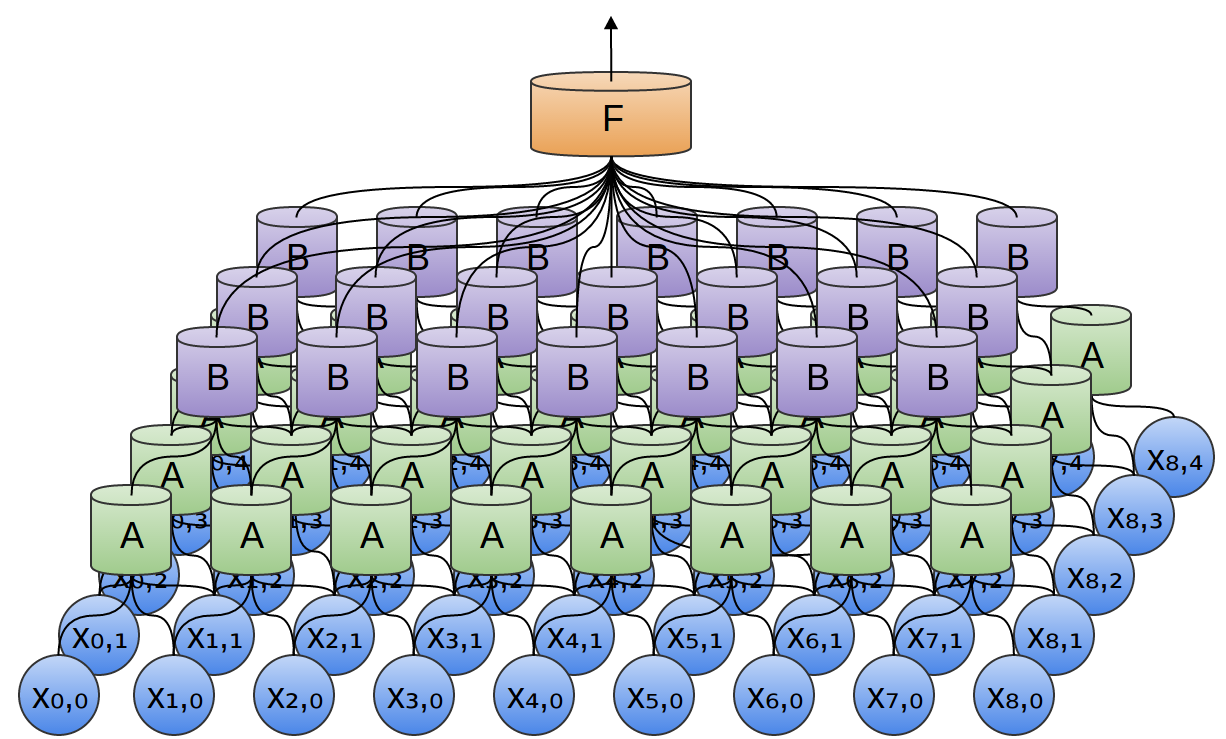
\includegraphics[width=\columnwidth]{sv}
	\caption{Свёрточная сеть}
\end{figure}

\item Сеть с прямым распространением сигналов. В ней запрещены циклы. Сначала сигнал передаётся на скрытый слой, затем на выходной слой и во внешнюю среду. Часто описывается в виде слоёного торта, где каждый слой состоит из входных, скрытых или выходных клеток. Клетки одного слоя не связаны между собой, а соседние слои обычно полностью связаны. Если у сети есть достаточное количество скрытых нейронов, она теоретически способна смоделировать взаимодействие между входным и выходными данными. Практически такие сети используются редко, но их часто комбинируют с другими типами для получения новых.

\begin{figure}
	\centering
	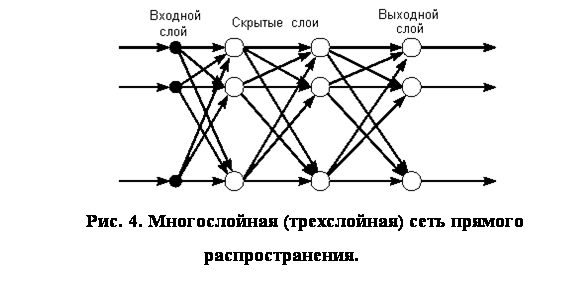
\includegraphics[width=\columnwidth]{pr}
	\caption{Первый пример сети с прямым распространением}
\end{figure}
\begin{figure}
	\centering
	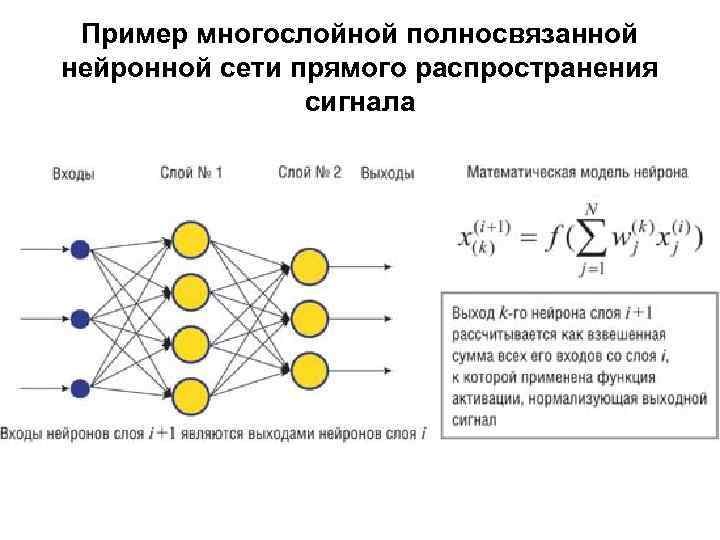
\includegraphics[width=\columnwidth]{pr2}
	\caption{Второй пример сети с прямым распространением}
\end{figure}

\item Рекуррентная сеть – сеть в которой возможны циклы. Здесь сигнал от входного может поступать на любой из скрытых слоёв из скрытого слоя или даже на предыдущий слой. Её можно представить в виде сети с прямым распространением сигнала во времени. В данной нс у каждого соединения есть свой вес, он же приоритет. Узлы в ней делятся на два типа, вводные узлы и узлы скрытые. Информация в рекуррентной нейронной сети передается не только по прямой, слой за слоем, но и между самими нейронами. Важной отличительной особенностью рекуррентной нейронной сети является наличие так званой «области внимания», когда машине можно задать определенные фрагменты данных, требующие усиленной обработки.

\begin{figure}
	\centering
	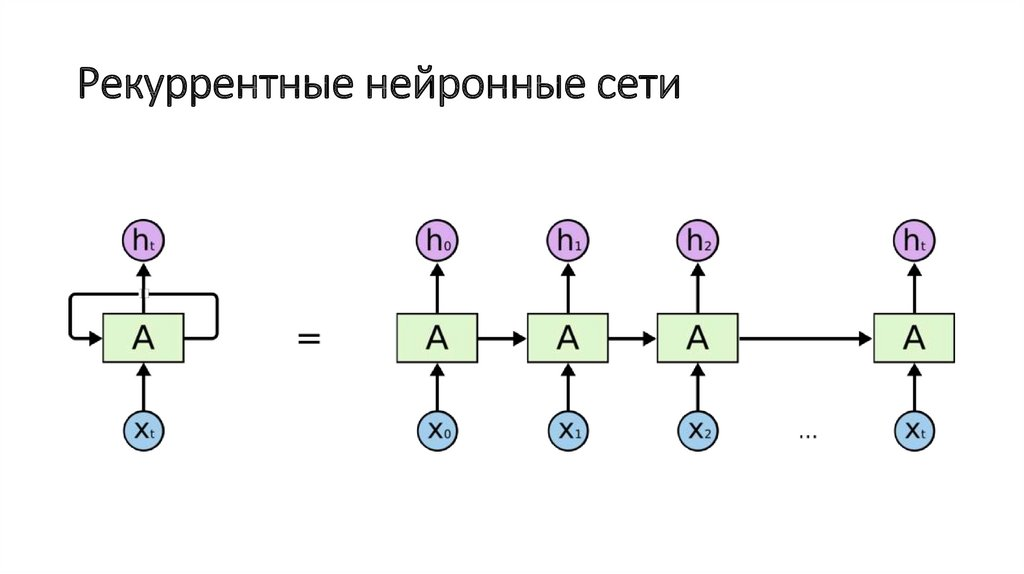
\includegraphics[width=\columnwidth]{rek}
	\caption{Пример рекуррентной сети}
\end{figure}
\begin{figure}
	\centering
	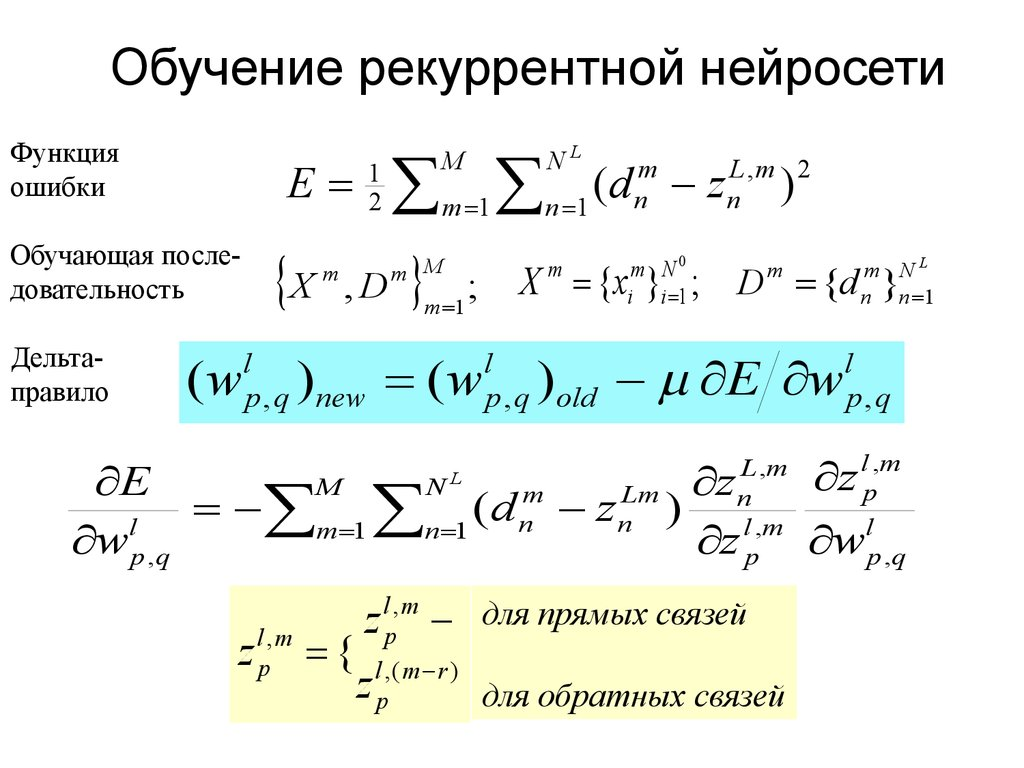
\includegraphics[width=\columnwidth]{rek2}
	\caption{Формульная запись}
\end{figure}

\end{enumerate}

Сети, у которых больше одного скрытого слоя называются глубокими нейронными сетями. 

Методы обучения:
\begin{enumerate}
	\item Обучение с учителем. Должен быть набор данных, которые подаются на вход нейронных сетей для которых заранее известен правильный ответ;
	\item Обучение без учителя. Есть данные, но правильный ответ для них заранее не известен;
	\item Обучение с подкреплением. Получает сигналы и ответы от внешней среды.
\end{enumerate}


 Методы поиска оптимальных весов 

Полное обучение. анализ ошибки на всех элементах данных, подсчёт направления градиента и только потом изменяем веса. Но если данных много, этот метод не будет эффективен.  

Онлайн обучение, это когда мы делаем шаг в сторону изменения, когда обработали один элемент данных или нескольких элементов данных (мини-выборки). В таких случаяхх на разных этапах обучения мы можем двигаться в разные стороны, в том числе, ошибка может увеличиваться. Но если данных много, а размер шага в сторону градиента маленький, то со временем мы дойдём до минимального значения функции ошибки. 

 Метод обратного распространения ошибки 

При обучении с учителем, нам нужно знать ошибку не только на выходном слое, но и на выходе всех скрытых слоёв и на входном слое. Зная ошибку на выходном слое, мы рассчитываем ошибку поочерёдно на скрытых слоях, затем на входном слое. Если мы знаем ошибку на выходе, мы можем получить ошибку на входе. Пусть у нас есть скрытый слой и мы получили ошибку на выходе. Если нейрон линейный, нам нужно взять значение на выходе из нейрона и умножить на вес этого выхода.  

Дельта правило (правило Видроу-Хоффа).
Определим ошибку $\delta$:

$\delta = y_0\medspace-\medspace y$
Здесь у нас $y_0y$ – это ожидаемый (истинный) вывод сети, а y – это реальный вывод (активность) выходного элемента. Помимо выходного элемента ошибки можно определить и для всех элементов скрытого слоя нейронной сети, об этом мы поговорим чуть позже.

Дельта-правило заключается в следующем – изменение величины весового коэффициента должно быть равно:

$\Delta w_{jk} = \eta\medspace\delta_k\medspace x_j$
Где $\etaη$ – норма обучения. Это число мы сами задаем перед началом обучения. $x_jx$ – это сигнал, приходящий к элементу k от элемента j. А $\delta_kδ$ – ошибка элемента k.

Таким образом, в процессе обучения нейронной сети на вход мы подаем образец за образцом, и в результате получаем новые значения весовых коэффициентов. Обычно обучение заканчивается, когда для всех вводимых образцов величина ошибки станет меньше определенной величины. После этого сеть подвергается тестированию при помощи новых данных, которые не участвовали в обучении. И по результатам этого тестирования уже можно сделать выводы, хорошо или нет справляется сеть со своими задачами.

С корректировкой весов все понятно, осталось определить, каким именно образом и по какому алгоритму будут происходить расчеты при обучении сети. Давайте рассмотрим обучение по алгоритму обратного распространения ошибки.

Алгоритм обратного распространения ошибки.
Этот алгоритм определяет два “потока” в сети. Входные сигналы двигаются в прямом направлении, в результате чего мы получаем выходной сигнал, из которого мы получаем значение ошибки. Величина ошибки двигается в обратном направлении, в результате происходит корректировка весовых коэффициентов связей сети. В конце статьи мы рассмотрим пример, наглядно демонстрирующий эти процессы.

Итак, для корректировки весовых значений мы будем использовать дельта-правило, которое мы уже обсудили. Вот только необходимо определить универсальное правило для вычисления ошибки каждого элемента сети после, собственно, прохождения через элемент (при обратном распространении ошибки).

$\delta_j = f{\Large{\prime}}(net_j)\medspace\cdot\medspace \sum_{k}{}{\delta_k\medspace w_{jk}}$. Функция $f(x)f(x)$ – это функция активности элемента. Давайте использовать логистическую функцию, для нее:
$f{\Large{\prime}}(net_j) = f(net_j)\medspace (1\medspace-\medspace f(net_j))$
Подставляем в предыдущую формулу и получаем величину ошибки:

$\delta_j = f(net_j)\medspace (1\medspace-\medspace f(net_j))\medspace \sum_{k}{}{\delta_k\medspace w_{kj}}$
В этой формуле:

$\delta_jδ  – ошибка элемента с индексом j$
k – индекс, соответствующий слою, который посылает ошибку “обратно”
$net_jnet$ 
j– комбинированный ввод элемента
$f(net_j)f(net)$ – активность элемента
Наверняка сейчас еще все это кажется не совсем понятным, но не переживайте, при рассмотрении практического примера все встанет на свои места! Собственно, давайте к нему и перейдем.

\begin{figure}
	\centering
	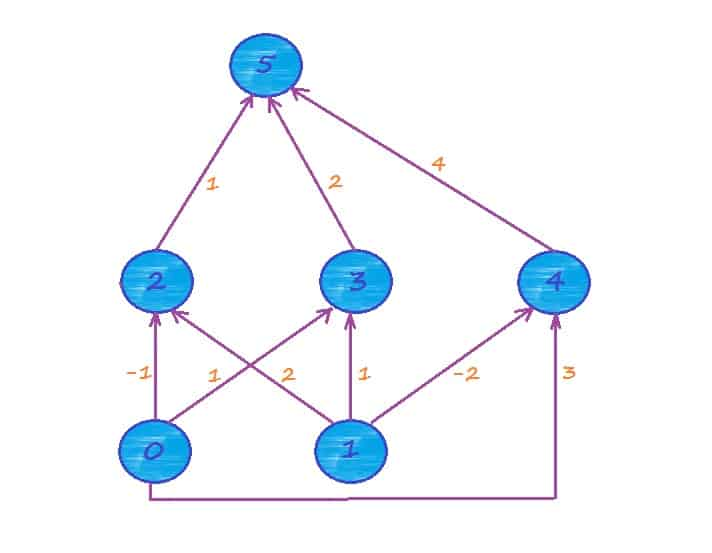
\includegraphics[width=\columnwidth]{weight}
	\caption{Распределение весов}
	\end{figure}

Методы оптимизации
\begin{enumerate}
	\item Нестеров Импульс
	Хорошее обсуждение импульса Нестерова дано вСуцкевер, Мартенс и др. «О важности инициализации и импульса в глубоком обучении» 2013,

	Основное отличие состоит в том, что в классическом импульсе вы сначала корректируете свою скорость, а затем делаете большой шаг в соответствии с этой 		скоростью (а затем повторяете), но в импульсе Нестерова вы сначала делаете шаг в направлении скорости, а затем вносите поправку в вектор скорости. на основе 	     нового местоположения (затем повторите).
	\item AdaGrad
	Momentum добавляет обновления наклона нашей функции ошибок и ускоряет SGD по очереди. AdaGrad адаптирует обновления к каждому отдельному параметру для 		выполнения больших или меньших обновлений в зависимости от их важности.
	Одним из главных преимуществ Adagrad является то, что он устраняет необходимость ручной настройки скорости обучения и приводит к большему прогрессу в слегка 	     наклонных направлениях.

	Основным недостатком AdaGrad является накопление квадратов градиентов в знаменателе: поскольку каждый добавленный член является положительным, накопленная 	   сумма продолжает расти в процессе обучения. Это, в свою очередь, приводит к уменьшению скорости обучения и в конечном итоге становится бесконечно малым, и в  	 этот 	момент алгоритм больше не может получать дополнительные знания.
	\item RMSProp
	Для невыпуклых задач AdaGrad может преждевременно снизить скорость обучения. Мы можем использовать экспоненциально взвешенное среднее для накопления 		градиента.
	\item Адам
	Адам представляет собой комбинацию RMSprop и импульса (аналогично, Надам относится к комбинации RMSprop и Нестерова импульса). Адам относится кадаптивная 	  оценка момента,и это самый популярный оптимизатор, используемый сегодня для нейронных сетей.

	Адам вычисляет адаптивные показатели обучения для каждого параметра. В дополнение к хранению экспоненциально убывающего среднего значения прошлых квадратов 	    градиентов vt, как Adadelta и RMSprop, Адам также сохраняет экспоненциально убывающее среднее значение прошлых градиентов, аналогично импульсу. 
\end{enumerate}


Список литературы:
\begin{enumerate}
	\item https://www.poznavayka.org/nauka-i-tehnika/neyronnyie-seti-ih-primenenie-rabota/
	\item https://microtechnics.ru/obuchenie-nejronnoj-seti-algoritm-obratnogo-rasprostraneniya-oshibok/
	\item https://habr.com/ru/post/318970/
	\item
\end{enumerate}
	
\end{document}
